\documentclass[12pt,a4paper]{article}
\usepackage[utf8]{inputenc}
\usepackage{amsmath}
\usepackage{amsfonts}
\usepackage{amssymb}
\usepackage{listings}
\usepackage{url}
\usepackage[bulgarian]{babel}
\usepackage{listings}
\usepackage{enumerate}
\usepackage{hyperref}
\usepackage[framemethod=tikz]{mdframed}
\usepackage{relsize}


\newcommand{\code}[1]{\texttt{#1}}

\lstset{breaklines=true} 


\author{\textit{email: kalin@fmi.uni-sofia.bg}}
\title{\textsc{Задачи за задължителна самоподготовка} \\
по \\
Обектно-ориентирано програмиране\\
\textit{Функции от високо ниво, шаблони, виртуални методи}}



\begin{document}
\maketitle


\begin{enumerate}

	
	\item Да се дефинира функция \code{double root ([подходящ тип]f, double a, double b, double e)}, където
	 $f:double \rightarrow double$ е непрекърсната и монотонна в интервала $[a,b]$ и притежава корен в него, а $e$ е положително число. Чрез използване на двоично търсене (\textit{bisection}), функцията \code{root} да намира приближение на корена на $f$ в интервала $[a,b]$ с грешка най-много $e$.

	\begin{mdframed}[hidealllines=true,backgroundcolor=gray!20]
	\relscale{0.75}
	Упътване:\\
	
	Установете дали функцията е растяща или намаляваща. Да приемем, че функцията е растяща. За намаляващи функции алгоритъмът е аналогичен. \\

	За всеки интервал $[a,b]$ имаме точно три възможни случая:\\

	\begin{center}
	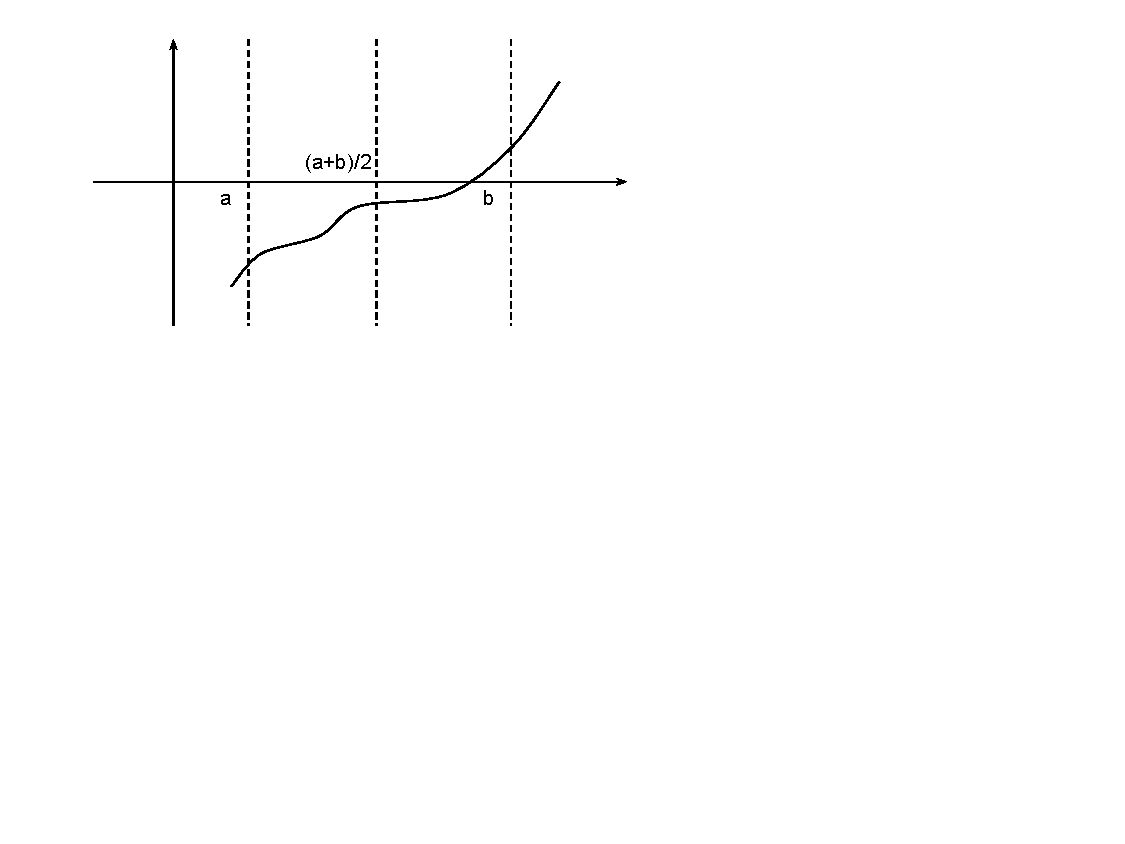
\includegraphics[width=14.0cm]{images/function}
	\end{center}

	\vspace{-180px}


	\begin{enumerate}
		\item $|f(\frac{a+b}{2})| < e$. В този случай приближението е намерено и то е $\frac{a+b}{2}$
		\item $f(\frac{a+b}{2}) < 0$. В този случай търсим корена на функцията в интервала $[\frac{a+b}{2},b]$
		\item $f(\frac{a+b}{2}) > 0$. В този случай търсим корена на функцията в интервала $[a,\frac{a+b}{2}]$
	\end{enumerate}
	

	\end{mdframed}

	\begin{itemize}
		\item Дефинирайте два варианта на функцията: итеративен и рекурсивен.
		\item Тествайте функцията \code{root} с поне два примера.
	\end{itemize}
	

	\item Да се дефинира функция \code{void zip (double a1[], double a2[], double res[], int n, [подходящ тип]f)}, където \code{a1}, \code{a2} и \code{res} са масиви с \code{n} на брой елементи, а \code{f} е функция от тип $f:double \times double \rightarrow double$. Като резултат от работата на функцията елементите на \code{res} да съдържат стойностите на функцията \code{f} върху съответните елементи на \code{a1} и \code{a2}, така че $res[i]=f(a1[i],a2[i])$ за $i=0..n-1$.
	\begin{itemize}
		\item Тествайте функцията с поне два примера.
	\end{itemize}
	\item Функцията \code{zip} от предишната задача да се преобразува до шаблон, така че масивите \code{a1}, \code{a2} и \code{res} да са от произволен тип \code{T}.
	\begin{itemize}
		\item Тествайте функцията с поне два примера.
	\end{itemize}
	\item Функцията \code{zip} от предишната задача да се преобразува до шаблон, така че всеки от масивите \code{a1}, \code{a2} и \code{res} да са от различни помежду си типове $T_1$, $T_2$ и $T_3$, а $f:T_1 \times T_2 \rightarrow T_3$.
	\begin{itemize}
		\item Тествайте функцията с поне два примера.
	\end{itemize}


	\item Към разработената на лекции йерархия от изчислими изрази да се добави клас, представящ оператора умножение.

	\item Към разработената на лекции йерархия от изчислими изрази да се добави клас \code{IfExpression}, представящ оператора разклонение (\code{if}). Операторът да зависи от три израза - \code{cond} (условие), \code{then\_expr} (израз в случай на вярно условие) и \code{else\_expr} (израз в случай на невярно условие). Стойността на оператора \code{if} да е стойността на израз \code{then\_expr} или \code{else\_expr} в зависимост от стойността на израза \code{cond}.\\

	Упътване: Ако се налага, може да разширите клас \code{Value} с метод за проверка на това дали съответната стойност е истинна или не.


	\begin{mdframed}[hidealllines=true,backgroundcolor=gray!20]
	\relscale{0.75}
	Пример:\\
	
	Нека \code{c}, \code{t} и \code {e} са обекти от някой наследник на клас \code {Expression}, като стойността на \code{c} е различна от 0. Тогава, при конструиране на обекта \code{ife} по следния начин: \code{IfExpr ife (\&c,\&t,\&e)}, то стойността на \code{ife.execute()} ще е същата като на \code{t.execute()}.
 
	\end{mdframed}

	\item Към разработената на лекции йерархия от изчислими изрази да се добави клас \code{ArithExpression}, представящ едновременно четирите аритметични оператора \code{+}, \code{*}, \code{-} и \code{/}. При конструиране на обектите да се уточнява конкретният оператор чрез един от символите \code{'+'}, \code{'*'}, \code{'-'} и \code{'/'}, съответно. Например, следният обект: \code{ArithExpr ae ('*',\&e1, \&e2)} да представя умножение на изразите, представени от \code{e1} и \code{e2}.

	\item Към разработената на лекции йерархия от изчислими изрази да се добави допустим тип на изразите \code{char}. Т.е. да се дефинира нов наследник на клас \code{Value}, представящ символния тип. 

	\item Към разработената на лекции йерархия от изчислими изрази да се добави допустим тип на изразите символен низ. Т.е. да се дефинира нов наследник на клас \code{Value}, представящ символен низ. 


\end{enumerate}







	\vspace{20px}


\end{document}

